%% Use the option review to obtain double line spacing
%% \documentclass[authoryear,preprint,review,12pt]{elsarticle}

%% Use the options 1p,twocolumn; 3p; 3p,twocolumn; 5p; or 5p,twocolumn
%% for a journal layout:
\documentclass[preprint,1p,times]{elsarticle}
%% \documentclass[final,1p,times,twocolumn]{elsarticle}
%% \documentclass[final,3p,times]{elsarticle}
%% \documentclass[final,3p,times,twocolumn]{elsarticle}
%% \documentclass[final,5p,times]{elsarticle}
%% \documentclass[final,5p,times,twocolumn]{elsarticle}

%% For including figures, graphicx.sty has been loaded in
%% elsarticle.cls. If you prefer to use the old commands
%% please give \usepackage{epsfig}

%% The amssymb package provides various useful mathematical symbols
\usepackage{amssymb}
\usepackage{tikz}
\usepackage{pgfplots}
%% The amsthm package provides extended theorem environments
%% \usepackage{amsthm}

%% The lineno packages adds line numbers. Start line numbering with
%% \begin{linenumbers}, end it with \end{linenumbers}. Or switch it on
%% for the whole article with \linenumbers.
%% \usepackage{lineno}

% \journal{Nuclear Physics B}

%% this is to export tikz graphics
\begin{document}

\begin{frontmatter}

%% Title, authors and addresses

%% use the tnoteref command within \title for footnotes;
%% use the tnotetext command for theassociated footnote;
%% use the fnref command within \author or \address for footnotes;
%% use the fntext command for theassociated footnote;
%% use the corref command within \author for corresponding author footnotes;
%% use the cortext command for theassociated footnote;
%% use the ead command for the email address,
%% and the form \ead[url] for the home page:
%% \title{Title\tnoteref{label1}}
%% \tnotetext[label1]{}
%% \author{Name\corref{cor1}\fnref{label2}}
%% \ead{email address}
%% \ead[url]{home page}
%% \fntext[label2]{}
%% \cortext[cor1]{}
%% \affiliation{organization={},
%%             addressline={},
%%             city={},
%%             postcode={},
%%             state={},
%%             country={}}
%% \fntext[label3]{}

\title{RtBot: a signal processing framework focused on early event detection}

%% use optional labels to link authors explicitly to addresses:
%% \author[label1,label2]{}
%% \affiliation[label1]{organization={},
%%             addressline={},
%%             city={},
%%             postcode={},
%%             state={},
%%             country={}}
%%
%% \affiliation[label2]{organization={},
%%             addressline={},
%%             city={},
%%             postcode={},
%%             state={},
%%             country={}}

\author{Robert Carcassés Quevedo}
\author{Eduardo Pérez Verdecia}
\author{Yuriel Núñez Jiménez}

% \affiliation{organization={},%Department and Organization
%            addressline={}, 
%            city={},
%            postcode={}, 
%            state={},
%            country={}}

\begin{abstract}
%% Text of abstract
RtBot framework is presented as a general purpose digital signal processing
framework focused on event detection.
\end{abstract}


\begin{keyword}
%% keywords here, in the form: keyword \sep keyword
digital signal processing \sep open source \sep event detection
\end{keyword}

\end{frontmatter}

%% \linenumbers

%% main text
\section{Introduction}
\label{}
RtBot is a general purpose digital signal processing framework focused on early event detection. 
It’s written in c++ and has been built with performance in mind.

Wrapper libraries exist for python, javascript (using wasm) and rust, and in the future we plan 
to support java and swift languages as well. In this sense RtBot can be easily adapted in any 
existing codebase, as it already provides interfaces to the most popular existing computer 
languages or new ones can be built for those missing languages using their native interface 
with c++. RtBot programs are very fast and have a low footprint, being able to run even in 
microcontrollers with very limited resources, such a raspberry pi pico or the esp32.

As a digital processing framework, it contains the common pieces found in such frameworks such as 
high and low pass filters, finite response filters, signal re-samplers and so on. 

As an event detector framework it is designed to give developers the tools to minimize the time 
difference between the moment when the event is detected and the moment when the event actually 
happened.


\section{Architecture}
\subsection{Modules}
RtBot framework is divided into a set of modules: \textit{core}, \textit{api} and \textit{std} ones. This 
list is likely to grow in the future and users can also extend it with their own 
private business model specific ones.


The \textit{core} module contains the general definitions and it does not depend on any 
other. You can write a program using only the core module, but you will have to 
write it in c++ and explicitly construct the operators and their connections. 


The \textit{api} module allows users to easily interact with the core module. For instance 
it can read RtBot programs saved in json format and construct the correspondent 
internal pipeline of operators at runtime. In this module is also where the 
external bindings are defined, giving a simplified api to run programs. If you are 
developing a web or desktop app, or even a mobile app, you will likely use this 
module. On the other hand, if you are building an embedded application for a 
microcontroller, including this module in your build will cause a large binary 
output that probably won’t fit on the device. In this case you will have to rely 
only on the core and std modules to make sure you produce binaries small enough.


The \textit{std} module represents a standard library of commonly used operators that can 
be used to build programs. Operators defined here are general purpose ones, like 
the inputs, resampler or finite response operators, which are ubiquitous used in 
any kinds of input signals. In practice this module and the core one will be the 
minimal components you will need in order to create some non trivial program.

\subsection{Inside the core}
An RtBot program expects a signal as input, which is a time-ordered stream of 
messages to be fed to it, one at the time, in what we call a program iteration. 
This iteration may or may not produce an output, which will be defined later.

A message is a tuple of timestamp and value. It is important to remark, even if 
obvious, that the timestamp in the message is the one used for any internal 
analysis, and not the time that the message arrives. RtBot has no clock inside or 
anything similar, so it has no way of counting real life time.


RtBot assumes the time inside a message to be an integer. The main motivation for 
this is that comparing two timestamps is more efficient and meaningful in this 
case than if we allow the timestamps to be of float type. This allows, for 
instance, to synchronize signals according to its timestamp in a much simplified 
and efficient way. This shall not, however, be a hurdle to adopt RtBot to process 
signals with fractionary timestamps, as a rescaling in the time dimension of the 
signal prior to sending it to the RtBot program will solve any type mismatch. This 
time scale, i.e. seconds or milliseconds, depends on the nature of the signal 
being processed and it is up to the programmer to decide which makes sense for the 
given type of signal.


Multidimensional signals can be processed by sending their components to specified input operators.

\subsection{Operators}
The main concept in the RtBot architecture is that of an operator. An operator 
it’s simply a computational unit that takes an input, transforms it and produces 
an output. Operators take messages as inputs and produce other messages as 
outputs. Remarkably, operators assume that they will receive messages with 
increasing timestamps, this is, ordered in time.


Operators can be connected with other operators, in a directed way, such that one 
operator can have children operators. If an operator has children then whenever it 
produces an output it will be sent to its children which will consider those 
messages as its own input, and so on. Operators may change the throughput of the 
stream they receive, producing any number of messages, or none, per each message 
it receives. In this sense they are also flow controllers, deciding when and what 
to forward to its children operators.


\subsubsection{Input}
An RtBot program is then this set of operators connected in a graph structure, 
a pipeline, where the external signal entry points are marked by the input 
operators. An input operator is just an operator that is designed to be a good 
intake of the external signal. Input operators are not mandatory but recommended 
entry points, as they perform sanity checks on the input signal before forwarding 
the message to others. For example, an input operator will discard new messages 
with timestamps prior or equal to the last message received, guaranteeing the time 
order in the messages it forwards.


\begin{figure}
    \label{fig:input operator action}
    \begin{center}
        
    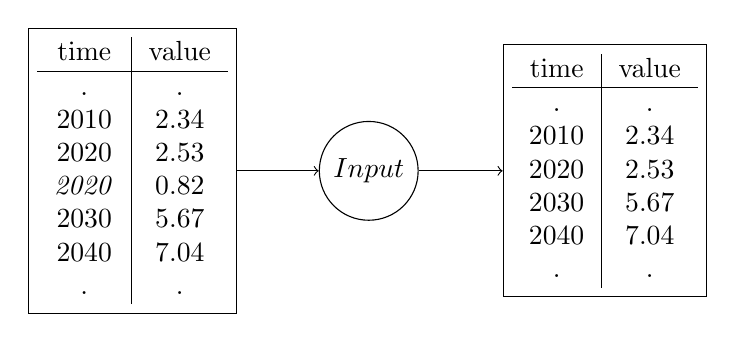
\begin{tikzpicture}[node distance={30mm}, main/.style = {draw, circle}, signal/.style = {draw}] 
    \node[main] (1) {$Input$}; 
    \node[signal] (2) [left of=1] {
            \begin{tabular}{ c | c }
            time & value \\ 
            \hline
            .    & . \\
            2010 & 2.34 \\  
            2020 & 2.53 \\  
            \textit{2020} & 0.82 \\  
            2030 & 5.67 \\  
            2040 & 7.04 \\  
            .    & . \\
            \end{tabular}
    };
    \node[signal] (3) [right of=1] {
            \begin{tabular}{ c | c }
            time & value \\ 
            \hline
            .    & . \\
            2010 & 2.34 \\  
            2020 & 2.53 \\  
            2030 & 5.67 \\  
            2040 & 7.04 \\  
            .    & . \\
            \end{tabular}
    }; 
    \draw[->] (2) -- (1);
    \draw[->] (1) -- (3);
    \end{tikzpicture} 
    \end{center}
    \caption{Action of the $Input$ operator in the incoming signal. Notice how the second message with the same timestamp $t=2020$ is ignored. The same would happen if the message timestamp would have been less than the previous one.}
\end{figure}


\subsubsection{Resamplers}

All operators that implement some math over their input assume that the messages 
it will receive are not only time ordered but also \textit{equidistant in time}, or \textit{equally
spaced in time}. We will call this type of signal a regular one, while those that
don't fulfill this will be named irregular. This is a strong assumption and it 
will likely be the case that input signals are irregular. This is why we have a
special set of operators called resamplers.

A resampler operator will take an irregular input signal and will produce a regular one. 
Internally, it will use the irregular signal as its source of truth, to find a realistic interpolation 
over the time grid points. The interpolation algorithm depends on the resampler
used. In practice this means that, while not strictly necessary, programs will 
start with input operators followed by resampler ones.

\begin{figure}[ht]
    \label{fig:resamplers}
    \begin{center}
        
    \begin{tikzpicture}[node distance={40mm}, main/.style = {draw, circle}, signal/.style = {}] 
    \node[main] (1) {$Resampler$}; 
    \node[signal] (2) [left of=1] {
        \begin{tikzpicture}
        \begin{axis}[width=6cm, xlabel={$t$}]
        \addplot[mark=*]
                coordinates {
                (10, 10.2)(20, 13.7)(23, 14.6)(55, 13.8)(60, 10.2)(70, 9.5)(73, 8.8)(120, 12.2)(130, 13.3)
                };
        \end{axis}
        \end{tikzpicture}
    };
    \node[signal] (3) [right of=1] {
        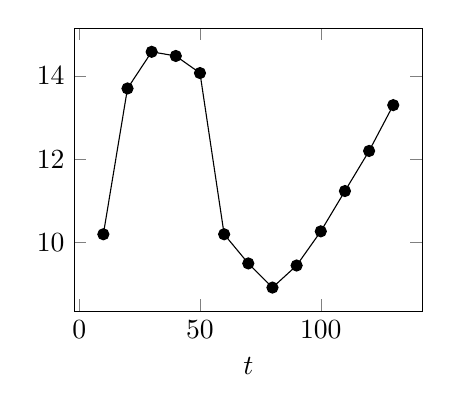
\begin{tikzpicture}
        \begin{axis}[width=6cm, xlabel={$t$}]
        \addplot[mark=*]
                coordinates {
                        (10, 10.2)(20, 13.7)(30, 14.58)(40, 14.48)(50, 14.07)(60, 10.2)
                        (70, 9.5)(80, 8.92)(90, 9.45)(100, 10.27)(110, 11.237531)(120, 12.200000)(130, 13.30)
                };
        \end{axis}
        \end{tikzpicture}
    }; 
    \draw[->] (2) -- (1);
    \draw[->] (1) -- (3);
    \end{tikzpicture} 
    \end{center}
    \caption{Action of a resampler operator. On the left an irregular signal, whose messages are not 
    uniformly distributed in time. On the right the output of the resampler operator: the produced stream
    of messages now are equidistant in time.}
\end{figure}

\begin{figure}[ht]
    \label{fig:resampler operator action table}
    \begin{center}
        
    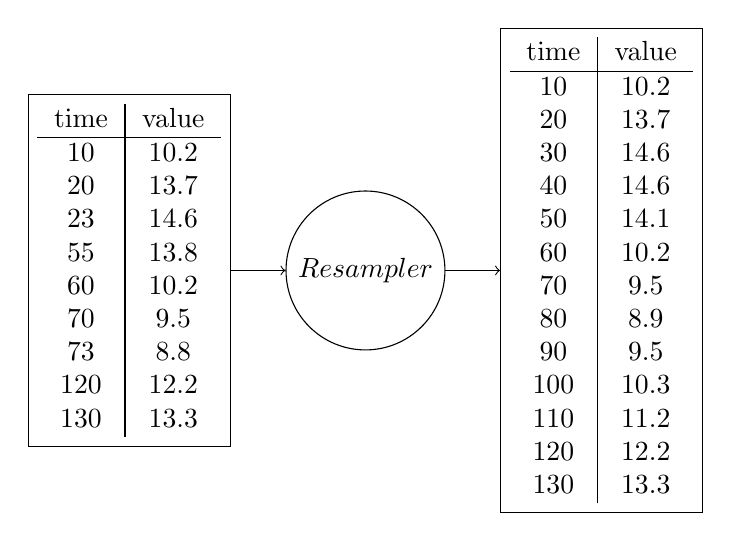
\begin{tikzpicture}[node distance={30mm}, main/.style = {draw, circle}, signal/.style = {draw}] 
    \node[main] (1) {$Resampler$}; 
    \node[signal] (2) [left of=1] {
            \begin{tabular}{ c | c }
            time & value \\ 
            \hline
            10 & 10.2  \\
            20 & 13.7  \\
            23 & 14.6  \\
            55 & 13.8  \\
            60 & 10.2  \\
            70 & 9.5  \\
            73 & 8.8  \\
            120 & 12.2  \\
            130 & 13.3  \\
            \end{tabular}
    };
    \node[signal] (3) [right of=1] {
            \begin{tabular}{ c | c }
            time & value \\ 
            \hline
            10 & 10.2 \\
            20 & 13.7 \\
            30 & 14.6 \\
            40 & 14.6 \\
            50 & 14.1 \\
            60 & 10.2 \\
            70 & 9.5 \\
            80 & 8.9 \\
            90 & 9.5 \\
            100 & 10.3 \\
            110 & 11.2 \\
            120 & 12.2 \\
            130 & 13.3 \\
            \end{tabular}
    }; 
    \draw[->] (2) -- (1);
    \draw[->] (1) -- (3);
    \end{tikzpicture} 
    \end{center}
    \caption{Action of the $Resampler$ operator in the incoming signal. 
    This is the same data presented in figure \ref{fig:resamplers} but in tabular format.
    Notice how the signal gets augmented by the resampler in order to fulfill the requirement
    of emitting regular time intervals. In this case the grid step is $\Delta t=10$.
    }
\end{figure}


\section{Use cases}
\subsection{Network traffic monitoring and statistics}
\subsection{Real time biofeedback}

In recent years we have experienced an explosion regarding wearable devices with the capacity to
constantly monitor our health. They can measure our heart rate, oxygen or sugar level in blood,
for instance. They constantly gather information about our bodies and can offer us feedback about
how we performed in certain activities, like how well did we sleep last night and can provide 
suggestions for our day accordingly.

Cheap wristbands, through its \textit{photoplethysmography} sensor, commonly known as PPG, are able to detect
heart pulses by injecting light into our tissue and measuring the luminosity changes of the reflected 
light. As the blood goes through our veins, it causes a measurable variation in this luminosity,
phenomena that can be used to infer our heart rate. From the patterns of variability of the heart 
rate in time, and also combining this with data of other sensors, many other things can be derived. 
The device can know whether we are running, sleeping or exercising, or even count how many repetitions 
of a given exercise type we have done in the gym.

There is one big caveat though: the measurements coming out of these devices often do not reflect reality 
and it is full of artifacts. There are many causes to this, like wearable devices not being used properly,
the quality of the sensor or having a low battery. But even the underlying physics itself of the measuring
mechanism is challenging if we want to get a reliable measurement. For example, the shape of the signal
coming out of a PPG sensor, the one that doctors put you on the tip of your finger when you first arrive
at urgent care, is considerably different, and less trustworthy,  than the signal coming out of an 
\textit{electrocardiogram} (ECG) equipment, which finds your heart rate by measuring the electrical signals that 
propagate over your body when the heart beats. The last one has sharper peaks compared with the first one, 
which are easier to detect, leading to better results. It comes to no surprise then that ECG equipment is 
the standard found in intensive care units.

In any case measurement's quality can be improved in many ways, like for instance improving the wearable 
analytics software capabilities. RtBot has been designed specifically to excel in this type of environment 
where cpu and memory are scarce. Its low resource usage footprint, together with the ecosystem productivity 
tools, allows it to easily create optimized algorithms to get best results per device type. It can help to 
improve peak detection as well as to flag signal parts as unusable, preventing the output of nonsense 
measurements. Moreover, due to the broad scope of the operators provided by the framework, it also opens 
the door for more complex analytics like secondary peak detection, pulse shape and more which can provide 
valuable information about our physical and even mental health.

The same argument applies to a large extent to professional health devices like ECG. RtBot can be used as 
well on their software to provide better analytics while providing a short development cycle from 
conceptualization to production phases.

\subsection{Trading bots}


%% The Appendices part is started with the command \appendix;
%% appendix sections are then done as normal sections
%% \appendix

%% \section{}
%% \label{}

%% If you have bibdatabase file and want bibtex to generate the
%% bibitems, please use
%%
%%  \bibliographystyle{elsarticle-num} 
%%  \bibliography{<your bibdatabase>}

%% else use the following coding to input the bibitems directly in the
%% TeX file.

\begin{thebibliography}{00}

%% \bibitem{label}
%% Text of bibliographic item

\bibitem{}

\end{thebibliography}
\end{document}
\endinput
%%
%% End of file `elsarticle-template-num.tex'.
